\documentclass[notheorems,compress,mathserif,table]{beamer}
%\useoutertheme[height=0.1\textwidth,width=0.15\textwidth,hideothersubsections]{sidebar}
\usecolortheme{whale}      % Outer color themes: whale, seahorse, dolphin
\usecolortheme{orchid}     % Inner color themes: lily, orchid
%\useinnertheme[shadow]{rounded}
%\setbeamercolor{sidebar}{bg=blue!50} \setbeamercolor{background
%canvas}{bg=blue!9}
\usefonttheme{serif}
\setbeamertemplate{navigation symbols}{}
%%------------------------���ú��---------------------------------------------------------------------
\usepackage{amsmath,amssymb}
\usepackage{graphicx}
\usepackage{listings}
%\DeclareGraphicsRule{*}{mps}{*}{}
\usepackage{xmpmulti}
\usepackage{algorithm,algorithmic}
\usepackage{times}
\usepackage{cite}
\usepackage{amssymb,amsmath,amsthm}
\usepackage{wasysym}
\usepackage{url}
\usepackage{subfigure}
\usepackage{pgf}
%\usepackage{colortbl,dcolumn}

%\usepackage{pgf,pgfarrows,pgfnodes,pgfautomata,pgfheaps}
%\logo{\includegraphics[height=0.09\textwidth]{wuda.pdf}}

%\renewcommand{\raggedright}{\leftskip=0pt \rightskip=0pt plus 0cm}
%\raggedright

%\def\hilite<#1>{%
%\temporal<#1>{\color{blue!35}}{\color{magenta}}%
%{\color{blue!75}}}

%\newcolumntype{H}{>{\columncolor{blue!20}}c!{\vrule}}
%\newcolumntype{H}{>{\columncolor{blue!20}}c}
%==================================�����==============================================================
%\newcommand{\upcite}[1]{\textsuperscript{\cite{#1}}}  %�Զ�������\upcite, ʹ�ο������������ϱ����
%\bibliographystyle{plain}
\newcommand{\domain}[1]{\mathbb{#1}}
\renewcommand{\algorithmiccomment}[1]{ /* #1 */}

\DeclareGraphicsRule{.gif}{eps}{.gif.bb}{`gif2eps #1}

\begin{document}
%%%%%%%%%%%%%%%%%%%%%%%%%%%%%%%%%%%%%%%%%%%%%%%%%%%%%%%%%%%%%%%%%%%%%%%%%%

\title{Spatial Correlation Estimation Using Maximum Likelihood}
\subtitle{(Summary)}
\author{Wai-Shing Luk%
  \thanks{{\tiny
      Email: luk@fudan.edu.cn}},
}

\frame{\titlepage}

\frame{\frametitle{Overview}
  \tableofcontents
}

%%%%%%%%%%%%%%%%%%%%%%%%%%%%%%%%%%%%%%%%%%%%%%%%%%%%%%%%%%%%%%%%%%%%%%%%%%%
\section{Problem Formulation}
\frame{\frametitle{Problem Formulation}
  \begin{itemize}
    \item
      Based on Geostatistics
    \item
      Gaussian process is assumed: $S(s_i) \sim N(\mu, \Sigma)$,
    \item
      where
      \begin{itemize}
         \item
            $\mu$: mean $\in \domain{R}^n$
         \item
            $\Sigma$: covariance matrix $\in \domain{R}^{n \times n}$
         \item
            $S$: location $\in \domain{R}^d$, where $d = 1 or 2$
      \end{itemize}
    \item
      Given samples $(y_1, y_2, \cdots, y_N) \in \domain{R}^n$
    \item
      For simplicity, assume $\mu=0$ (zero mean), without adding noise
%%      minimize $\log \det \Sigma^{-1} - \mathrm{Trace}(\Sigma^{-1}\cdot Y)$
    \item
      $\Sigma_{ij} = \mathrm{Corr}(s_i,s_j)$
    \item
      Correlation function must be positive definite, i.e. 
      $\sum_i\sum_j a_i a_j \mathrm{Corr}(s_i, s_j) \ge 0$
  \end{itemize}
}

\begin{frame}
\frametitle{What the data can tell you?}
      \pgfputat{\pgfxy(0,-3.0)}{\pgfbox[left,base]{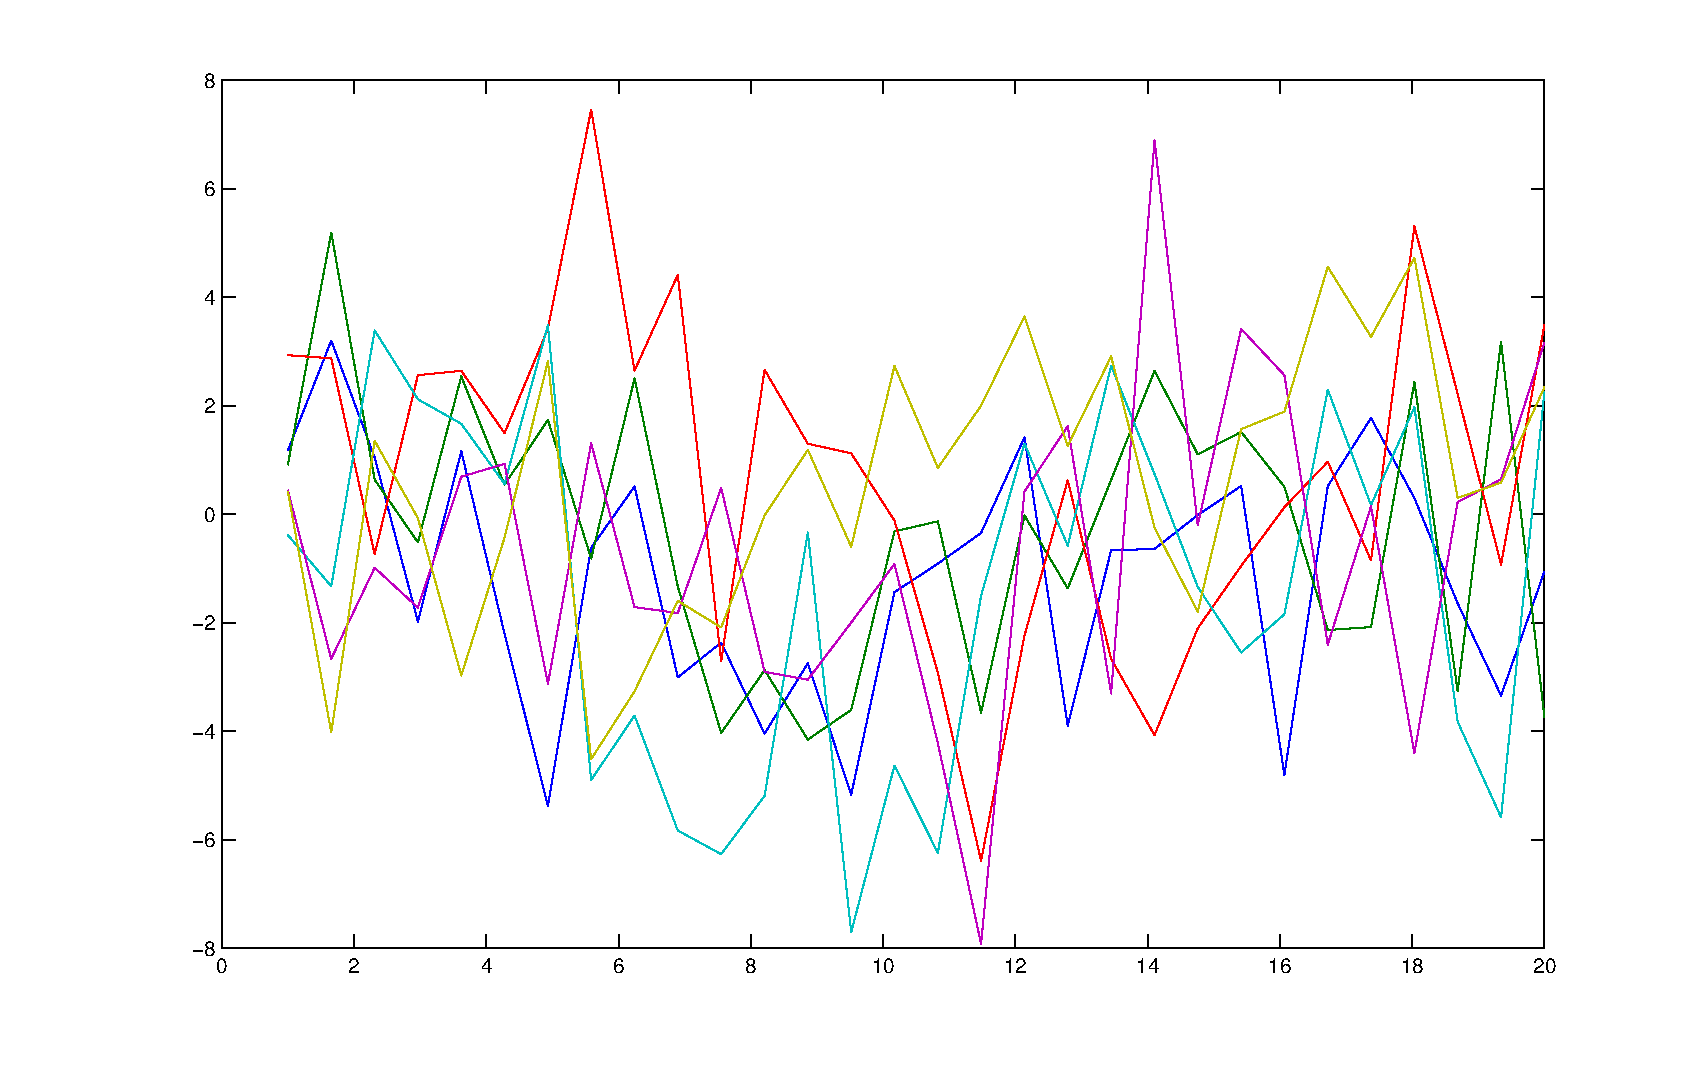
\includegraphics[width=\textwidth]{exp1d_data}}}
Note: pseudo-random numbers can't be perfect.
\end{frame}

\section{Non-parametric estimation}
%%%%%%%%%%%%%%%%%%%%%%%%%%%%%%%%%%%%%%%%%%%%%%%%%%%%%%%%%%%%%%%%%%%%%%%%%
\frame{\frametitle{Non-Parametric Maximum Likelihood Estimation}
  \begin{itemize}
  \item
    Estimate $\Sigma$ directly
    \begin{itemize}
    \item
      Useful for anisotropic problems, or justifying the isotropic assumption.
    \item
      The problem can be formulated as a convex programming.
    \item
      Disadvantage: slow if $n$ is large.
    \end{itemize}
  \item
    Negative log-likelihood function (ignore scaling and constant term)
    \[
      {\cal L}(\Sigma) = \log\det\Sigma^{-1} + \mathrm{Tr}(\Sigma^{-1} \cdot Y)
    \]
    where
    \begin{itemize}
    \item
      $Y = (1/N) \sum_{i=1}^N y_i y_i^{T}$
    \end{itemize}
  \item
    The first term is concave, whereas the second term is convex.
  \item
    However, let $S = \Sigma^{-1}$, the function becomes convex in term of $S$
    %% minimize $\log \det \Sigma^{-1} - \mathrm{Trace}(\Sigma^{-1}\cdot Y)$
  \item
    Note: other possible formulation: Whittle likelihood
  \end{itemize}
}

%%%%%%%%%%%%%%%%%%%%%%%%%%%%%%%%%%%%%%%%%%%%%%%%%%%%%%%%%%%%%%%%%%%%%
\begin{frame}
\frametitle{Non-Parametric Maximum Likelihood Estimation}
  \begin{columns}
    \begin{column}{0.5\textwidth}
      \begin{itemize}
       \item
	 Convex formulation:
	 \begin{itemize}
	   \item
	     \begin{equation*}
	       \begin{array}{cl}
		 \mbox{maximize}  & \log\det S - \mathrm{Tr}(S \cdot Y) \\
		 \mbox{subject to}& S \succeq 0, 
	       \end{array}
	     \end{equation*}
	   \item
             $\Sigma \leftarrow (S^*)^{-1}$
	 \end{itemize}
      \item
        $S$ represents the conditional correlation between two locations
        on the condition that all other locations are known.
      \item
        It is straightforward to be implemented in CVX.
      \end{itemize}
   \end{column}

    \begin{column}{0.5\textwidth}
      \pgfputat{\pgfxy(0,-3.0)}{\pgfbox[left,base]{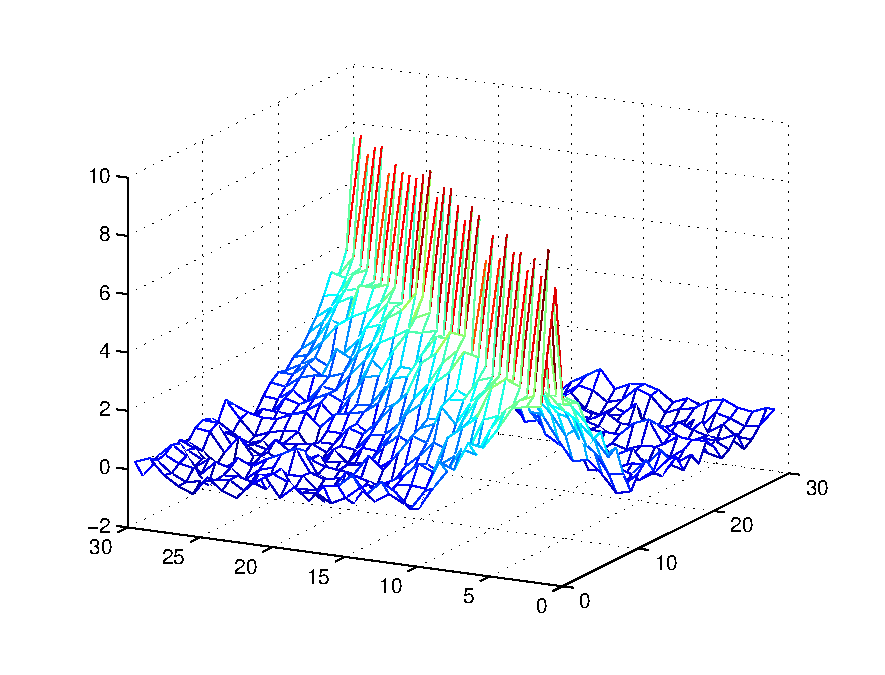
\includegraphics[width=\textwidth]{corr_mtrx}}}
    \end{column}
  \end{columns}
\end{frame}

%%%%%%%%%%%%%%%%%%%%%%%%%%%%%%%%%%%%%%%%%%%%%%%%%%%%%%%%%%%%%%%%%%%%%%
\begin{lstlisting}


  n = size(Y,1);
  cvx_begin sdp
    variable S(n,n) symmetric
    maximize(log_det(S) - trace(S*Y))
    subject to 
       S >= 0;
  cvx_end
  Sig = inv(S);
\end{lstlisting}

\section{Parametric estimation}
%%%%%%%%%%%%%%%%%%%%%%%%%%%%%%%%%%%%%%%%%%%%%%%%%%%%%%%%%%%%%%%%%%%%%%%
\begin{frame}
  \frametitle{Parametric Estimation}
  \begin{itemize}
  \item
    Usually for isotropic problems and the correlation model is known in prior,
    e.g. Mat\'{e}rn family. 
  \item
    The correlation matrix $\Sigma$ is a function of parameters,
    making the formulation non-convex.
  \item
    {\it ... Skipped the details}
  \end{itemize}
\end{frame}


\section{Semi-parametric estimation}
%%%%%%%%%%%%%%%%%%%%%%%%%%%%%%%%%%%%%%%%%%%%%%%%%%%%%%%%%%%%%%%%%%%%%%%
\begin{frame}
  \frametitle{Semi-parametric Estimation}
  \begin{itemize}
  \item
    An unknown function is curve-fitted by $\sum_i p_i \Phi_i(h)$,
    where
    \begin{itemize}
    \item
      $p_i$: scalar parameter
    \item
      $\Phi_i:$ basis function
    \end{itemize}
  \item
    Choice of $\Phi_i(h)$:
    \begin{itemize}
    \item
      $J_i(h)$: Bessel function, \\ 
                advantage: positive definite {\em if and only if} $p_i \ge 0$
		for all $i$. \\
                disadvantage: difficult to choose $i$, computational expensive.
    \item
      $B_i(h)$: B-spline function, \\
                advantage: shapes are easier to control, \\
                e.g. monotonicity ($p_i \ge p_{i+1}$); \\
		disadvantage: not guarantee positive definite
    \item
      $\cos((2\pi i/N)h)$: cosine functions
    \end{itemize}
  \item
    Choice of the unknown function:
    \begin{itemize}
    \item
      Correlation function $\rho(h)$:
    \item
      Spectral density function (using Fourier transform) [???]
    \item
      Kernel function (using moving average) [???]
    \item
      Inverse correlation function (???)
    \end{itemize}
  \end{itemize}
\end{frame}

\begin{frame}
  \frametitle{Concave-Convex Proceduce}
  \begin{itemize}
  \item
    Let $\rho(h) = \sum_i^m p_i \Phi_i(h)$ and $p = (p_1, \cdots, p_m)$.
  \item
    Then $\Sigma$ is an affine function of $p$:
    \[
      \Sigma = p_1 F_1 + p_2 F_2 + \cdots + p_m F_m 
    \]
    and hence preserves the convexity of the Log-likelihood function.
  \item
    Utilize the following inequality:
    \[
      \log\det\Sigma \ge \log\det\Sigma_0 + 
         \mathrm{Tr}(\Sigma_0^{-1} (\Sigma - \Sigma_0))
    \]
   \item
     For each iteration, solve the following minimization problem:
     \begin{equation*}
       \begin{array}{cl}
	 \mbox{minimize} & 
            \mathrm{Tr}(\Sigma_k^{-1}\Sigma) + \mathrm{Tr}(S\cdot Y) \\
	 \mbox{subject to}& 
            \left[
               \begin{array}{cc}
                  \Sigma & I \\
                    I    & S
                \end{array}
             \right] \succeq 0, 
       \end{array}
     \end{equation*}
   \item
     Note: may get local minimum only. Double check your result.
  \end{itemize}
\end{frame}

%%%%%%%%%%%%%%%%%%%%%%%%%%%%%%%%%%%%%%%%%%%%%%%%%%%%%%%%%%%%%%%%%%%%%%%%%%%
\begin{lstlisting}


  S_k = inv(Sig_k);
  for i=1:nx, t(i) = trace(S_k*F(:,:,i)); end
  cvx_begin sdp
    variables p(nx) % coefficents of B-spline
    variable S(n,n) symmetric
    variable Sig(n,n) symmetric

    minimize(t'*p + trace(S*Y))
    subject to
      for i=1:nx-1,
        p(i) >= p(i+1); % nonincreasing
      end
      % Sig = sum( F(:,:,i)*p(i) )
      Sig == reshape(reshape(F,n*n,nx)*p, n, n);
      [Sig  I;
        I   S ] >= 0;
  cvx_end
\end{lstlisting}

%%%%%%%%%%%%%%%%%%%%%%%%%%%%%%%%%%%%%%%%%%%%%%%%%%%%%%%%%%%%%%%%%%%%%
\begin{frame}
\frametitle{Concave-Convex Estimation}
  \begin{columns}
    \begin{column}{0.5\textwidth}
      \begin{itemize}
       \item
         Initialization: $\Sigma_0 = Y$
       \item
         For each iteration $k$, 
	 \begin{itemize}
	   \item
	     solve the convexified problem with $\Sigma_k$.
	   \item
             $\Sigma_{k+1} \leftarrow \Sigma^*$
	 \end{itemize}
      \end{itemize}
      \textcolor{red}{Red line:} theoretical correlation function.
   \end{column}

    \begin{column}{0.5\textwidth}
      \pgfputat{\pgfxy(0,-3.0)}{\pgfbox[left,base]{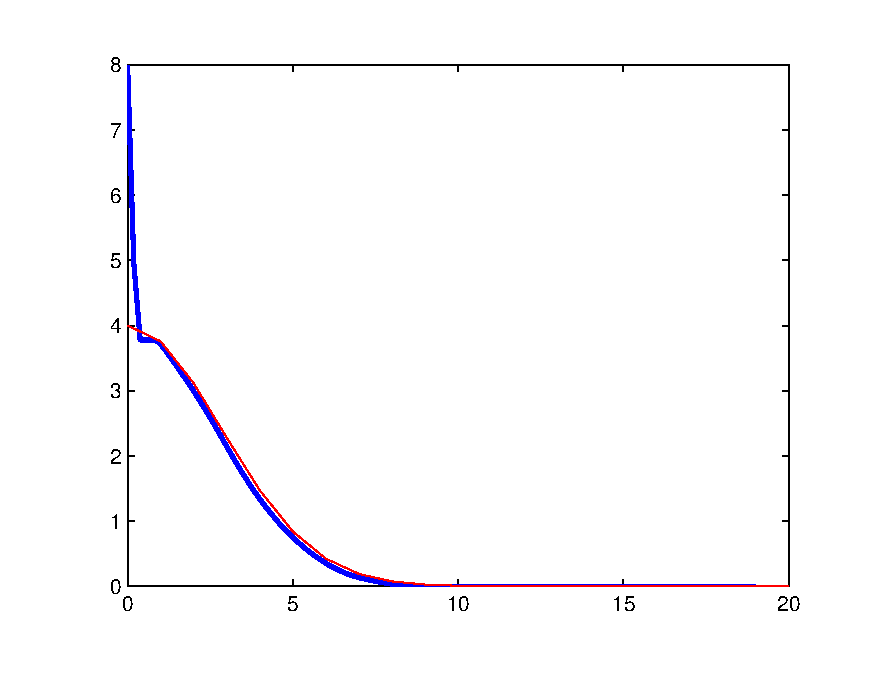
\includegraphics[width=\textwidth]{corr_fn}}}
    \end{column}
  \end{columns}
\end{frame}


%%%%%%%%%%%%%%%%%%%%%%%%%%%%%%%%%%%%%%%%%%%%%%%%%%%%%%%%%%%%%%%%%%%%%
\begin{frame}
\frametitle{Inverse Correlation function}
  \begin{columns}
    \begin{column}{0.5\textwidth}
      \begin{itemize}
       \item
	 Convex formulation:
	 \begin{itemize}
	   \item
	     \begin{equation*}
	       \begin{array}{cl}
		 \mbox{maximize}  & \log\det S - \mathrm{Tr}(S \cdot Y) \\
		 \mbox{subject to}& 
                                \begin{array}{l}
                                    S \succeq 0, \\
                                    S = q_1 F_1 + q_2 F_2 + \cdots
                                \end{array} 
	       \end{array}
	     \end{equation*}
	   \item
             $\Sigma \leftarrow (S^*)^{-1}$
	 \end{itemize}
      \item
        It is straightforward to be implemented in CVX.
      \end{itemize}
   \end{column}

    \begin{column}{0.5\textwidth}
      \pgfputat{\pgfxy(0,-3.0)}{\pgfbox[left,base]{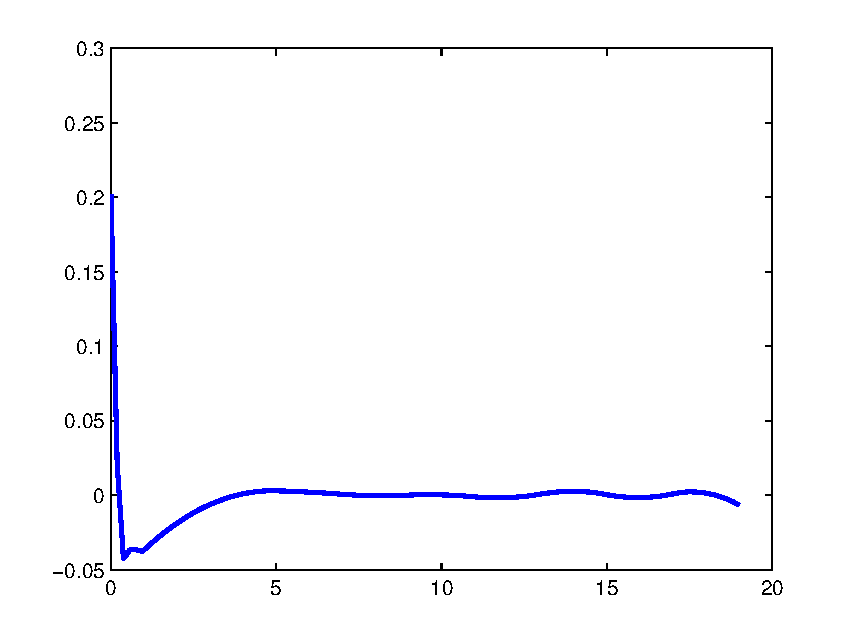
\includegraphics[width=\textwidth]{inv_corr_fn}}}
    \end{column}
  \end{columns}
\end{frame}

%%%%%%%%%%%%%%%%%%%%%%%%%%%%%%%%%%%%%%%%%%%%%%%%%%%%%%%%%%%%%%%%%%%%%%%%%%%
\begin{lstlisting}


cvx_begin sdp
  variable q(nx)  % coefficents of B-spline
  variable S(n,n) symmetric
  minimize(-log_det(S) + trace(S*Y))
  subject to
    S >= 0;
    S == reshape(reshape(F,n*n,nx)*q, n, n);  
cvx_end
sq = spmak(knotsx, q, nx);
Sig = inv(S);
\end{lstlisting}


%%%%%%%%%%%%%%%%%%%%%%%%%%%%%%%%%%%%%%%%%%%%%%%%%%%%%%%%%%%%%%%%%%%%%
\begin{frame}
  \frametitle{Problem of Using Inverse Correlation Function}
  \begin{columns}
    \begin{column}{0.5\textwidth}
      \begin{itemize}
      \item
	Can't satisfy all three conditions at the same time:
	\begin{itemize}
	\item
	  $\Sigma = p_1 F_1 + p_2 F_2 + \cdots$
        \item
	  $S = q_1 F_1 + q_2 F_2 + \cdots$
	\item
	  $\Sigma \cdot S = I$
	\end{itemize}
      \end{itemize}
    \end{column}
    
    \begin{column}{0.5\textwidth}
      %%% \pgfputat{\pgfxy(0,-3.0)}{\pgfbox[left,base]{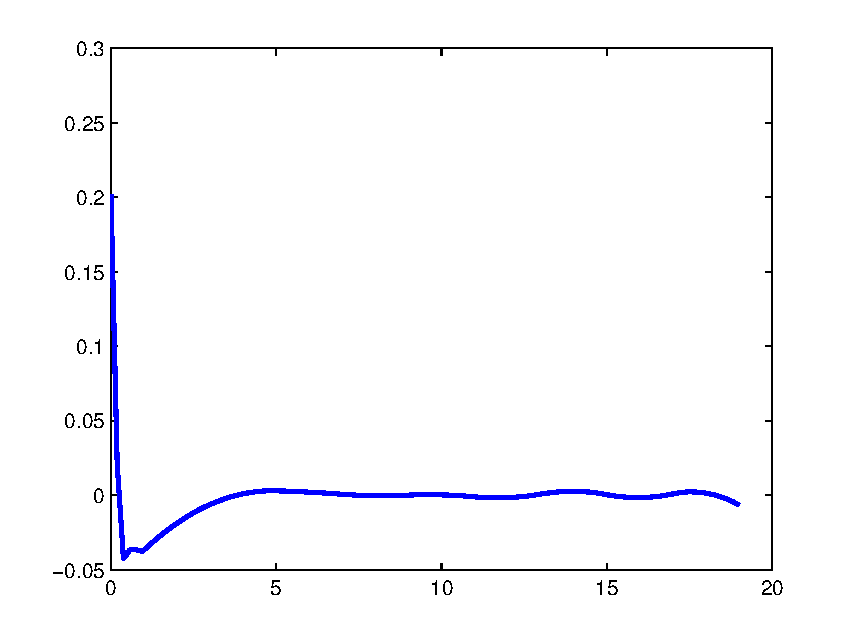
\includegraphics[width=\textwidth]{inv_corr_fn}}}
      \pgfputat{\pgfxy(0,-3.0)}{\pgfbox[left,base]{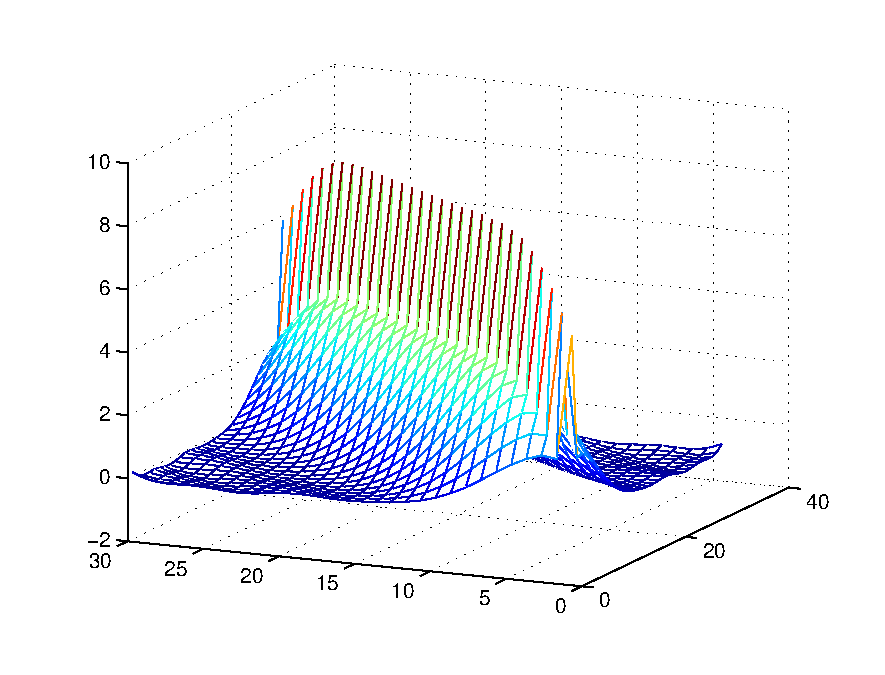
\includegraphics[width=\textwidth]{corr_mtrx_by_inv}}}
    \end{column}
  \end{columns}
\end{frame}

%%%%%%%%%%%%%%%%%%%%%%%%%%%%%%%%%%%%%%%%%%%%%%%%%%%%%%%%%%%%%%%%%%%%%
\begin{frame}
  \frametitle{Some properties of Correlation Function}
  \begin{columns}
    \begin{column}{0.5\textwidth}
      \begin{itemize}
      \item
	Positive definiteness: equivalent to its Fourier transform $\gt 0$.
      \item
	Monotonicity: correlation decreased with distance.
      \item
        Non-negativeness: only have positive correlation.
      \end{itemize}
      Note: B-spline can control the shapes easily.
    \end{column}
    
\end{frame}


\end{document}
